\justifying
\noindent

\section{Sensor Technology}
This section of the paper will focus on sensor technology, Specifically in LCD Display and Infrared Imaging (Thermography). This section will include brief introduction, system mechanism, and real-life application for each type of categories. \\

\subsection{Liquid-Crystal Display (LCD)}
\noindent Liquid-Crystal Display has become one of the major usage in any display application due to its low power consumption than its competitor such as LED or Cathode Ray Tube (CRT). The application of LCD range from basic 8-bit numbering display to high-pixel colour display such as television. liquid crystal refers to the state of a matter that has two distinct melting point which combines both two states of matter, solid and liquid \cite{AnonymousLCDApplications}\cite{Gurski2005DisplayOverview}. The application of an electric or magnetic field allows the manipulation of molecules orientation to a predicted manner which become the basis of LCD, moreover, the principle of LCD is to block the light from the backlight emitted \cite{Gurski2005DisplayOverview}.\\

\begin{figure}[!ht]
\begin{center}
%    
  \begin{subfigure}[b]{0.4\textwidth}
    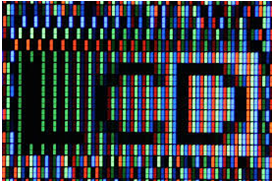
\includegraphics[height=4cm]{Figures/LCD_general.PNG}
  \end{subfigure}
  %
  \begin{subfigure}[b]{0.35\textwidth}
    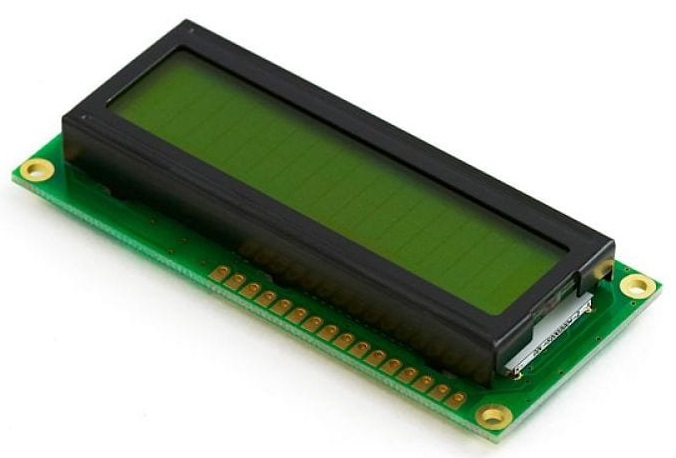
\includegraphics[height=4cm]{Figures/LCD_BASIC.jpg}
  \end{subfigure}
%  
  \caption{An LCD Representation \cite{Gurski2005DisplayOverview} (left) and basic character LCD \cite{AnonymousBasicSystems} (right).}
    \label{fig:basic lcd}
\end{center}
\end{figure}


\noindent A typical construction of typical LCD shown in figure \ref{fig:LCD structure} below. The first structure is the backlight source followed with bottom polarisers which perpendicular to each other in purpose of molecules alignment when current is applied. Thin-film-transistor (TFT) and glass substrate which are one of liquid crystal, and colour filter and black matrix are placed in between the polarisers \cite{AnonymousLCDApplications}. \\ 

\noindent The LCD works by untwisting the molecules by applying current to the liquid-crystal. This allows the angle of light passes through the molecules of the bottom polarised filter and changed the angle of top polarising filter. All this mechanism allows the light to pass the small amount of light through the particular area of the LCD, therefore creating a more dark region compared to others.

\begin{figure}[!ht]
    \centering
    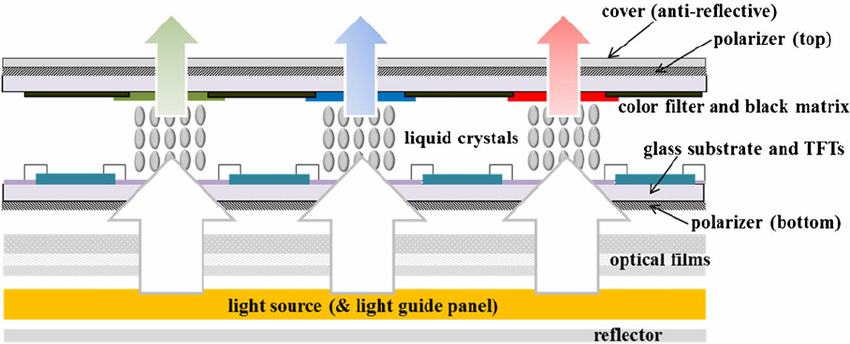
\includegraphics[scale=0.4]{Figures/LCD_Typical structure.png}
    \caption{A Typical structure of an LCD \cite{Park2013EfficiencyPrograms}}
    \label{fig:LCD structure}
\end{figure}

\subsubsection{Aircraft Navigation Panel \& General Purposes}
The most common use of an LCD panel is to aid and support the navigation by applying a simple display to a coordinate or frequency. In the modern technologies, LCD has developed into a  high-definition (HD) colour display which allows advance applications (camera view, GPS, etc)  rather than showing a basic character. In modern aircraft such as Airbus A350 and Boeing 787 use large multi-functional display units \cite{AnonymousTouchAirbus} and this system are usually based on full colour matrix LCD.  The more advanced LCD also includes touch-control interface which could simplify the aircrews and instruments interactions during all flight phase \cite{AnonymousTouchAirbus}. Figure \ref{fig:avionics 5inc} below shows 5 inch LCD avionics display in an aircraft cockpit and general avionics LCD composition.\\

\begin{figure}[!ht]
\begin{center}
%    
  \begin{subfigure}[b]{0.4\textwidth}
    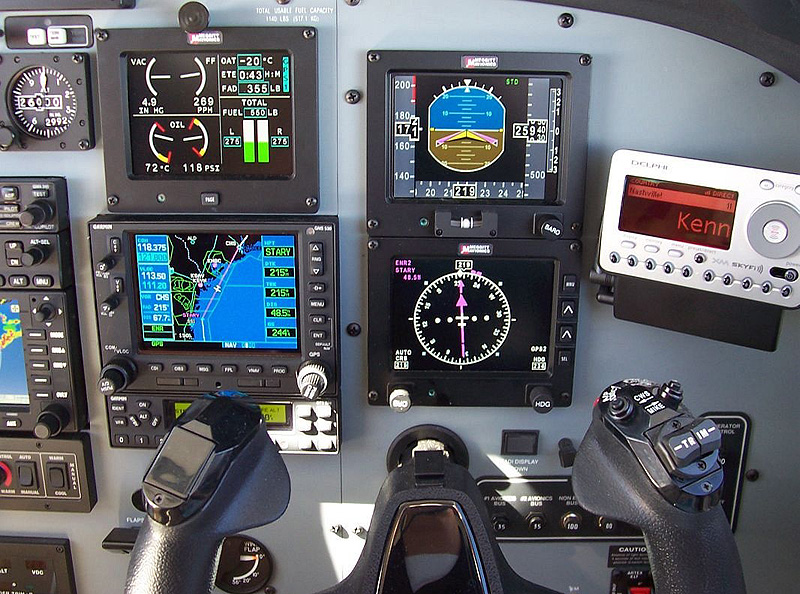
\includegraphics[height=5cm]{Figures/LCD_Avionics_5inch.jpg}
  \end{subfigure}
  %
  \begin{subfigure}[b]{0.35\textwidth}
    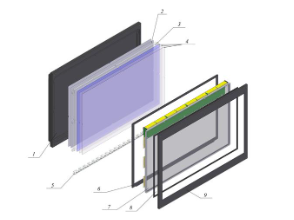
\includegraphics[height=5cm]{Figures/LCD_avionics_composition.PNG}
  \end{subfigure}
%  
  \caption{LCD application of avionics display on a Piper aircraft cockpit \cite{Anonymous5LCD} (left) and Avionics LCD Composition diagram \cite{Alimova2020MethodsApplications} (right).}
    \label{fig:avionics 5inc}
\end{center}
\end{figure}

\noindent Figure \ref{fig:avionics 5inc} right shows a typical aviation LCD MDU which displays various flight information. However, a regular LCD has a high reflection of light fluxes which increases bias and ambiguity of a pilot to the instruments in a high ambient light operation. Therefore, the modern LCDs are also coated with anti reflection coating which could reduce the reflection factor to 0.1\% \cite{Livada2012AFVCriteria}.\\

\noindent Additionally, the cost of LCD has become more economical over the years due to the manufacturing development. Therefore, the application of LCD has broaden from basic general use such as television, automatic teller machine(ATM), to car Navigation system. Figure \ref{fig:LCD var app} below shows other broad applications of LCD in real-life.\\

\begin{figure}[!ht]
    \centering
    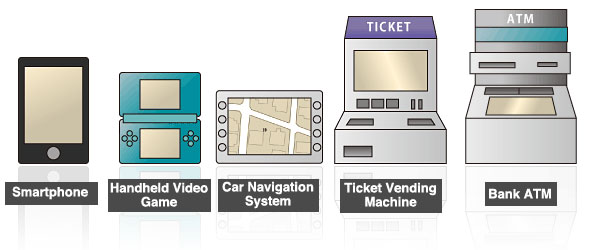
\includegraphics[scale = 0.6]{Figures/LCD_various app.jpg}
    \caption{Various Real Life Applications of LC Displays \cite{AnonymousHowEIZO}.}
    \label{fig:LCD var app}
\end{figure}

\subsection{Infrared Imaging (Thermography)}

An object with temperature above absolute zero (0K) in space emits electromagnetic waves called thermal radiation which generated due to the kinetic energy of a charged particles in an object \cite{Stumper2015ThermalAviation}. The amount of this radiation is proportional to object's temperature, also, thermal radiation emit both visible and infrared light. A standard camera responds to the visible light, however, thermographic camera/unit respond to the infrared radiation which presented as a false colour to represent temperature of a matter \cite{AnonymousThermographyEngineering}. \\

\begin{figure}[!ht]
    \centering
    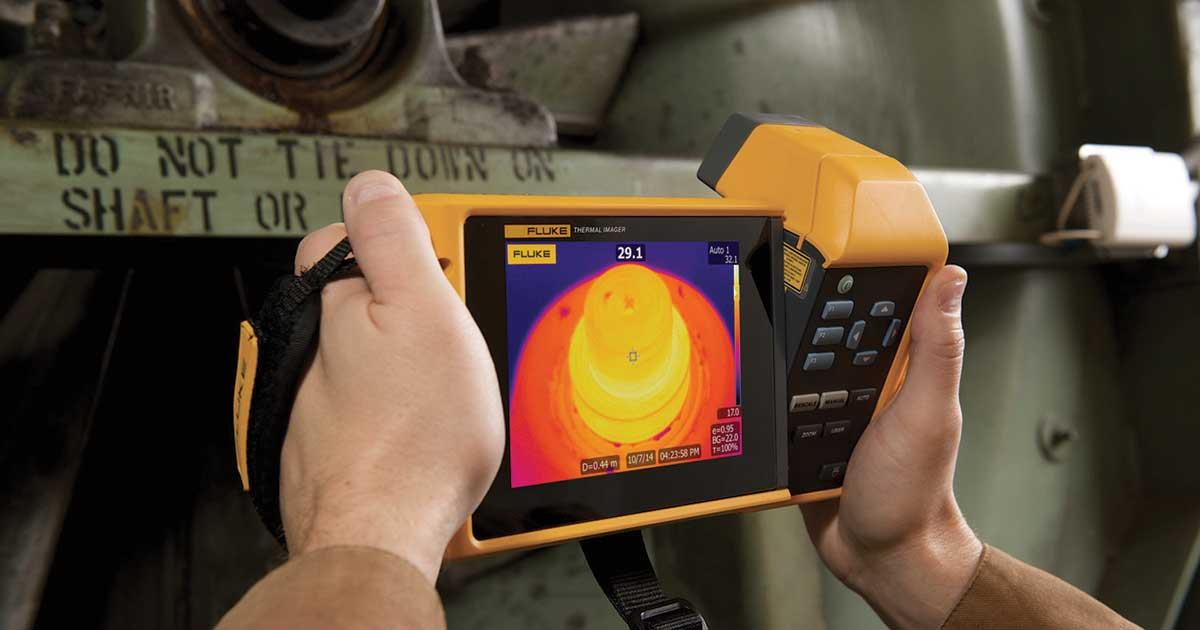
\includegraphics[scale=0.3]{Figures/IR_example_false image.jpeg}
    \caption{Example of a thermographic camera producing false image to convey material temperature \cite{TroutInfraredPlant}.}
    \label{fig:basic IR}
\end{figure}

\noindent However, thermographic system or camera accuracy depends on other external factors (e.g. surrounding temperature). Therefore, to achieve an effective use of thermography, adjustment such as; focus, emissivity, reflective temperature, and thermal tuning settings are required \cite{TroutInfraredPlant}. This technology create possibilities for limitless applications and user-friendly thermography is developing in respect of technology to be used by all user level.\\

\subsubsection{Aviation Industry}
In the aviation industry, infrared or thermography camera is used in wide range of applications, from material evaluation to surveillance system. In modern aircraft, infrared camera is used for Enhanced Vision System (EVS) which allows pilot vision of ground terrain in a low light operation. The infrared camera installed in an aircraft can project object with various temperature which includes object with various dimension. This technology allows pilot to see runways markings, taxiways, terrains, etc, and highway which increase pilot awareness in a low light or extreme condition (e.g. fog or rain) \cite{Stumper2015ThermalAviation}. Figure \ref{fig:EVS system} shows the pilot's vision of an aircraft's EVS system view.  \\

\begin{figure}[!ht]
\begin{center}
%    
  \begin{subfigure}[b]{0.4\textwidth}
    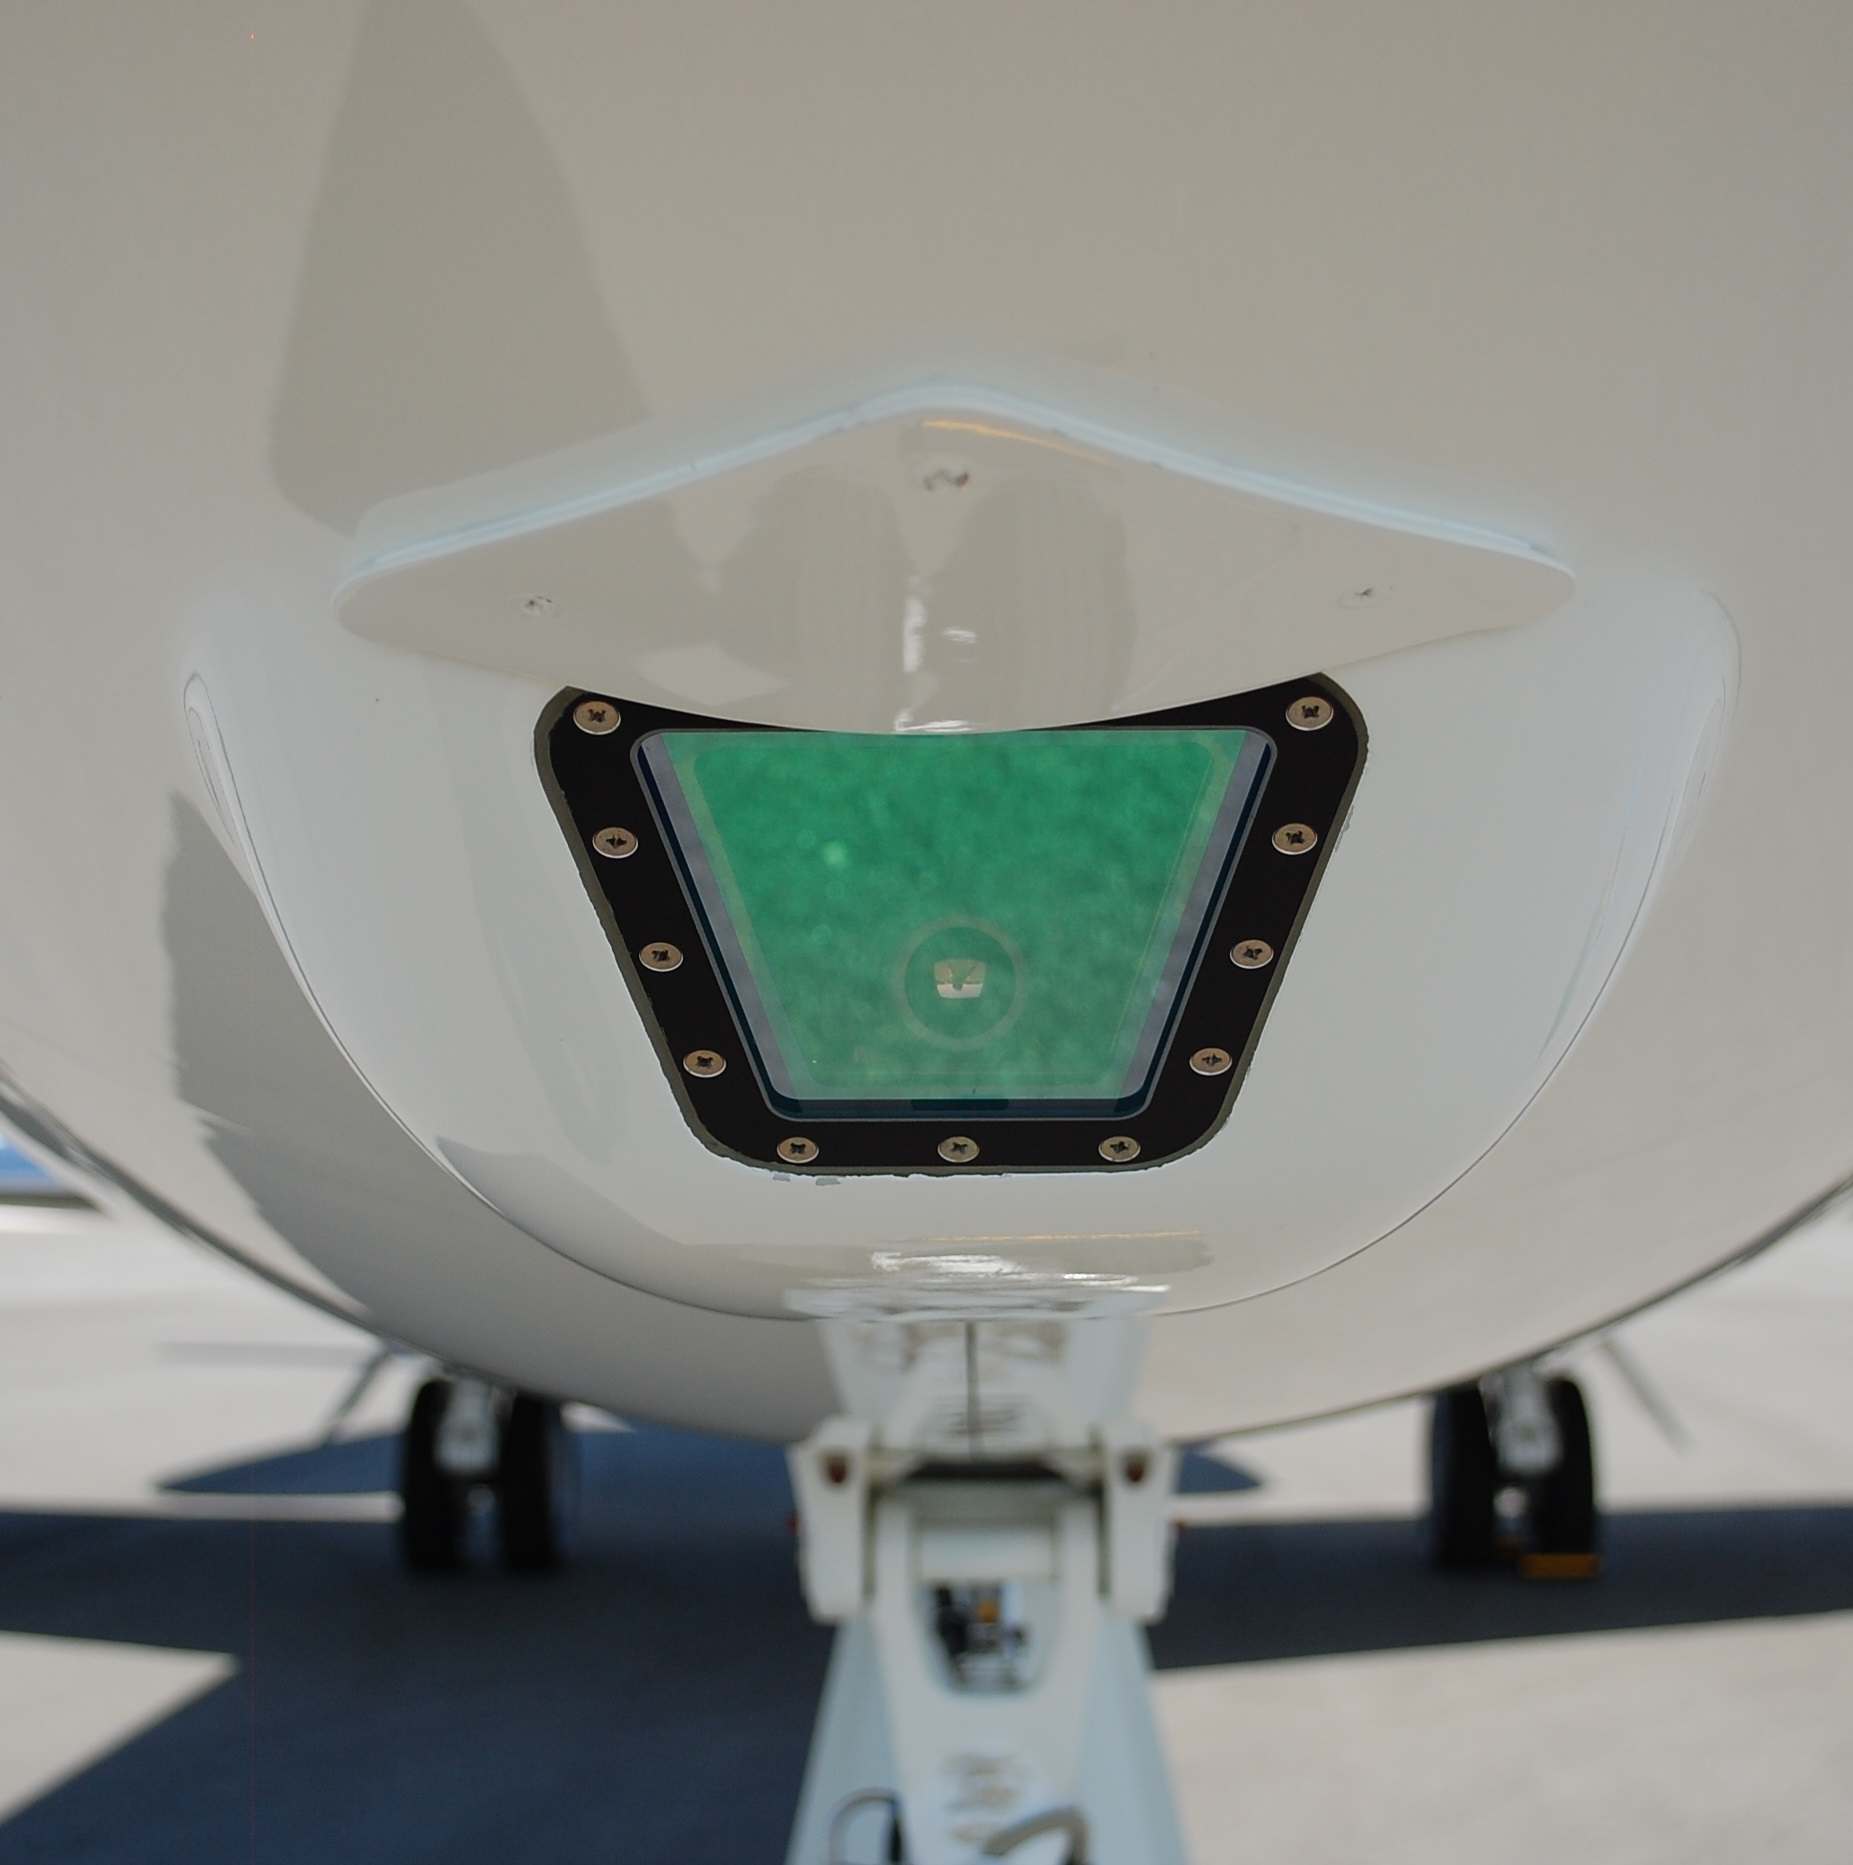
\includegraphics[height=5cm]{Figures/IR_IR camera install.jpg}
  \end{subfigure}
  %
  \begin{subfigure}[b]{0.5\textwidth}
    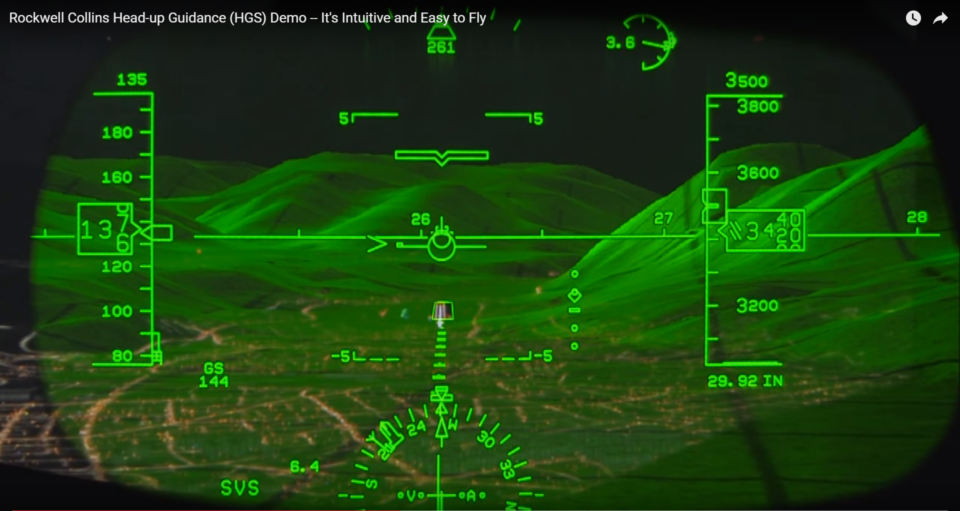
\includegraphics[height=5cm]{Figures/IR_EVS view.png}
  \end{subfigure}
%  
  \caption{An infrared camera installed on an aircraft \cite{AnonymousEnhancedWikipedia} (left) and cockpit view of EVS at night \cite{FehrmBjornsAnalysis} (right).}
    \label{fig:EVS system}
\end{center}
\end{figure}

\noindent Due to the rise of COVID-19 pandemic, airports around the world have been trying to conduct mass screening to detect passengers with potential virus. Generally, the first stage of mass screening is temperature measurement. With hundreds of thousands of travellers passing through an airport, the application of infrared thermography (IRT) is deemed to be the most efficient and accurate. In the airport IRT is one of the most valuable tools for non contact, noninvasive, and rapid screening of body temperature.  The sensitivity of IRT in an airport could range from 40 to 89.4\% depending on various circumstances such as; ambient temperature, humidity, ventilation, and performance differential \cite{Sun2017ApplicationsStations}. Figure \ref{fig:airport_IR} shows the difference between visual image view, thermal image, and mixing (isotherm display).\\

\begin{figure}[!ht]
    \centering
    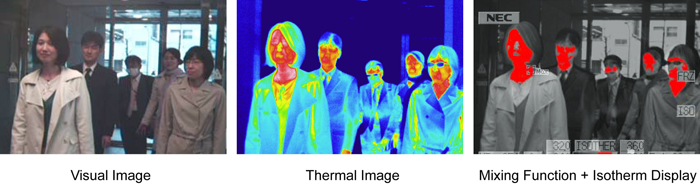
\includegraphics[scale=0.6]{Figures/IR_airport.jpg}
    \caption{Application of thermography as a mass temperature monitoring at the airport \cite{AnonymousBodyCO.LTD.}}
    \label{fig:airport_IR}
\end{figure}

\noindent Another advanced application of thermography in aviation is non-destructive material testing (NDT). This technology has been used for years in the aircraft industry and it has an advantage of inspecting large area in efficient and safe manner without to have physical or visual aspect of the aircraft body \cite{Ibarra-CastanedoInfraredMaterials}. Infrared NDT allows inspection of  the most common anomalies found on aircraft body such as; disbond, water ingress, core crushing, and delaminations. To detect these anomalies, a heat flow is applied to the body part by conducting energy in pulsed form or harmonic modulated such as halogen lamps \cite{Stumper2015ThermalAviation}. The body temperature is recorded using thermographic camera which then will be analysed using mathematical analysis \cite{Anonymous2013InformationImprovement}.

\begin{figure}[!ht]
    \centering
    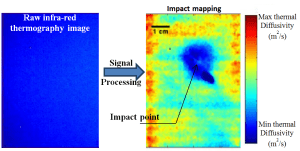
\includegraphics[scale=1.2]{Figures/IR_NDT.png}
    \caption{Illustration of raw infrared thermography image processed to impact mapping by using signal processing \cite{Non-destructiveLab}.}
    \label{fig:ndt_av}
\end{figure}
 
